\documentclass[conference]{IEEEtran}
\usepackage{bm}
\usepackage{cite}
\usepackage{ragged2e}
\usepackage{graphicx}
\usepackage{amsmath}
\usepackage{amssymb}
\usepackage{amsthm}
\usepackage{algorithm}
\usepackage{algpseudocode}
\usepackage{enumitem}
\usepackage{etoolbox}
\usepackage{mathrsfs}
\usepackage{subfig}
\usepackage{array}
\usepackage{cases}
\usepackage{dsfont}
\usepackage{optidef}
\usepackage{cleveref}

\allowdisplaybreaks
\newtheorem{theorem}{Theorem}
\newtheorem{lemma}{Lemma}
\newtheorem{definition}{Definition}
\setlength{\columnsep}{0.21in}
\makeatletter
\newcommand\fs@betterruled{%
  \def\@fs@cfont{\bfseries}\let\@fs@capt\floatc@ruled
  \def\@fs@pre{\vspace*{0.03in}\hrule height.8pt depth0pt \kern2pt}%
  \def\@fs@post{\kern2pt\hrule\relax}%
  \def\@fs@mid{\kern2pt\hrule\kern2pt}%
  \let\@fs@iftopcapt\iftrue}
\floatstyle{betterruled}
\restylefloat{algorithm}
\makeatother
\renewcommand{\arraystretch}{1.2}
\begin{document}
\title{Final Report for Wireless Mobile Network}
\author{\IEEEauthorblockN{Chia-Hung Lin, Chun-Yen Lee, Lu-Yo Kuo}
\IEEEauthorblockA{
Department of Electrical Engineering, National Taiwan University \\
b06504016@ntu.edu.tw, b06203017@ntu.edu.tw, b06502153@ntu.edu.tw}}
\maketitle

\section{Introduction}
In this final project, our goal is to evaluate the performance of the D2D system and the multicast system. In the first section, we simulate the D2D system and the traditional cellular systems. We compare the characteristic and conclude the differences between these two systems. In the second section, we simulate the point-to-multipoint (PTM) multicast network and the single frequency multicast network (SFN). We compute the average data rates for both multicast networks and explain how the number of mobile stations influence the resource efficiency.
\section{HW5}
\subsection{System Model}
The system is about Device to Device (D2D) systems. The distance between receive and transmission pair is fixed to $100m$. Both transmission user equipment (UE) and receive UE are in the central cell. There are $75$ UE pairs in the system.
\begin{figure}[htbp]
    \centering
    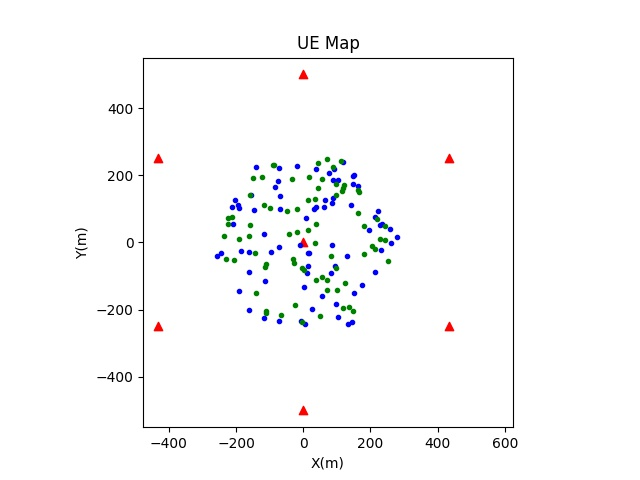
\includegraphics[width=0.45\textwidth]{fig1_1.jpg}
    \caption{The simulated map for UEs}
    \label{fig:ue_map}
\end{figure}


In \Cref{fig:ue_map}, the green point indicates the receive UE, and the blue point indicates the transmission UE. The red triangle indicates the base stations in the system.
\subsection{Basic D2D Topology Simulation}
\subsubsection{Simulation Parameters}
In the system, the bandwidth is $10$MHz, the temperature is $27^\circ$C, the power of the base stations is $23$dBm, the power of UEs in $0$dBm, the antenna gain of receive and transmit is both $0$dB. The UE height is $1.5$m, and the base station height is $51.5$m. The path loss model is Two-ray-ground model, which can be written as
\begin{equation}\label{eqn:two_ray}
    g(d) = P_t \times \dfrac{Gh_t^2h_r^2}{d^4}
\end{equation}
where $P_t$ is the transmit power, and $G$ is the total gain, $h_t$ and $h_r$ are height of transmit and receive antennas respectively.
\subsubsection{PMF for Uplink SINR}
In the uplink scenario, as shown in \Cref{fig:uplink_sinr}, the SINR of the uplink signal is between $60$ to $130$ dB, which is very large. This can be explained by the assumption that there is no interference in the uplink transmission.
\begin{figure}[htbp]
    \centering
    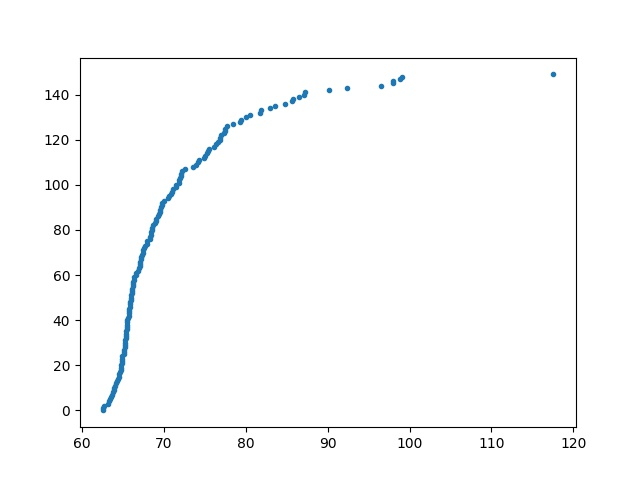
\includegraphics[width=0.45\textwidth]{fig1_2_a.jpg}
    \caption{CDF for Uplink SINR}
    \label{fig:uplink_sinr}
\end{figure}

\subsubsection{PMF for Downlink SINR}
In the downlink scenario, as shown in \Cref{fig:downlink_sinr}, the SINR of the downlink signal is between $0$ to $70$ dB.
\begin{figure}[htbp]
    \centering
    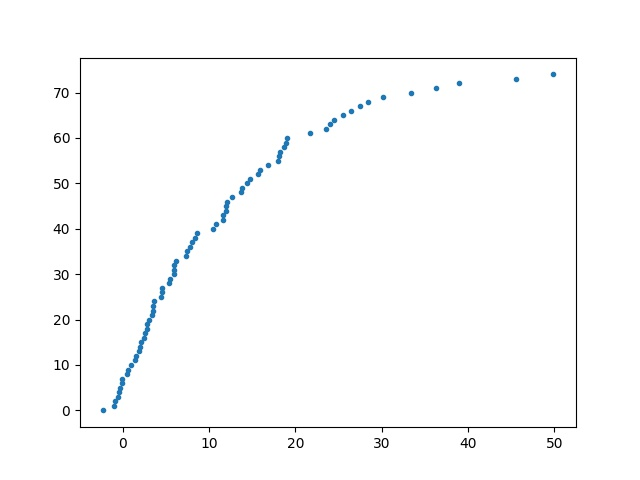
\includegraphics[width=0.45\textwidth]{fig1_2_b.jpg}
    \caption{CDF for Downlink SINR}
    \label{fig:downlink_sinr}
\end{figure}
Although the power of the downlink is from the base station, the SINR is smaller than the uplink signal. This difference is mainly caused by the different presumption of the uplink and downlink transmission signal, where the uplink signal is hypothesized to be interference-free, and the downlink signal is assumed to be interference by the signal from other base station.
\subsubsection{Total Throughput of the Downlink transmission}
By the simulation, the total throughput is approximately $2.58$ Gbps.
\subsubsection{PMF of the D2D SINR}
In D2D system, as shown in \Cref{fig:d2d_sinr}, the SINR of the D2D signal is mostly between $-65$ to $-25$ dB.

\begin{figure}[htbp]
    \centering
    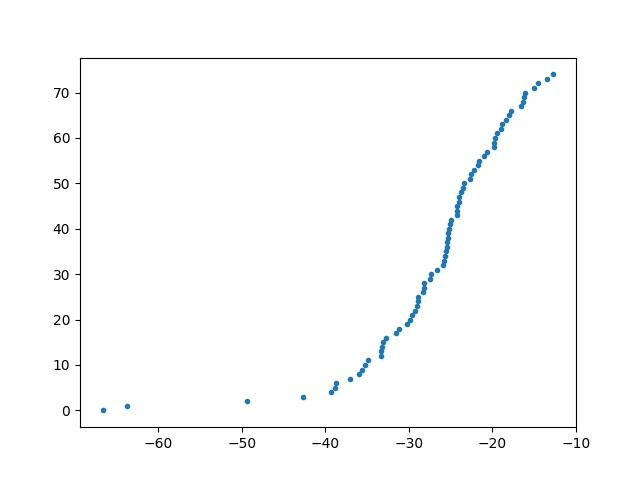
\includegraphics[width=0.45\textwidth]{fig1_4.jpg}
    \caption{CDF for D2D SINR}
    \label{fig:d2d_sinr}
\end{figure}
The huge gap of SINR between D2D systems and up/down link systems is caused by various reasons. Mostly, it is caused by the interference signal of other D2D pairs.
\subsubsection{Total Throughput of the D2D system}
By the simulation, the total throughput is approximately $490$ kbps.
\subsubsection{Total Throughput with different number of D2D pairs}
As seen in \Cref{fig:d2d_num}, when the number of D2D pairs increases, the total throughput is likely to decline.

\begin{figure}[htbp]
    \centering
    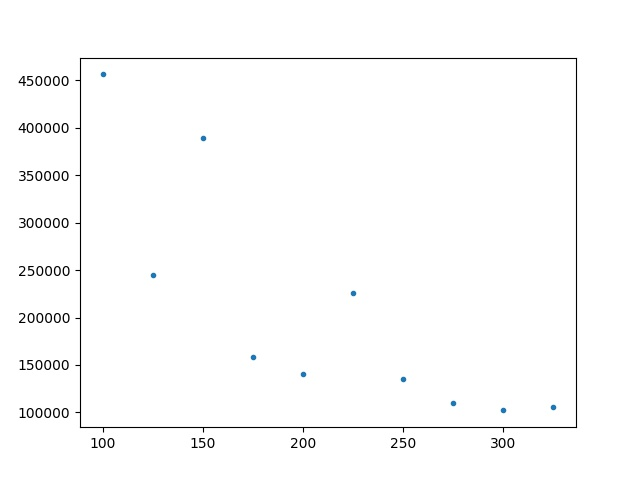
\includegraphics[width=0.45\textwidth]{fig1_6.jpg}
    \caption{Total Throughput vs. Number of D2D Pair}
    \label{fig:d2d_num}
\end{figure}
 This phenomenon is generated by the interference of other UEs. If the number of pairs increases, the distance between the receive UE and other transmit UE is very likely to be close, hence the increase of interference. However, the curve is not strictly decreasing for several reasons, the fluctuation is mainly caused by the difference of distance between the D2D pairs.
\subsection{Basic D2D Topology Discussion}
\subsubsection{Under which conditions does D2D transmission method perform better than cellular transmission method? Why?}
In the simulation, the distance is set to be $200$m, which is very large. Because of the huge distance, the SINR is small compared to the cellular signal. If the transmit and receive pair become closer, D2D systems can take advantage of the proximity, so total throughput can exceed cellular systems. In our bonus simulation, we set the distance to $10$m, and we discovered that the total throughput became $3.97$Gbps, which is faster than the cellular systems. We also re-plot \Cref{fig:d2d_num} by resetting the distance to $10$m. The result is in \Cref{fig:d2d_num_bonus}.
\begin{figure}[htbp]
    \centering
    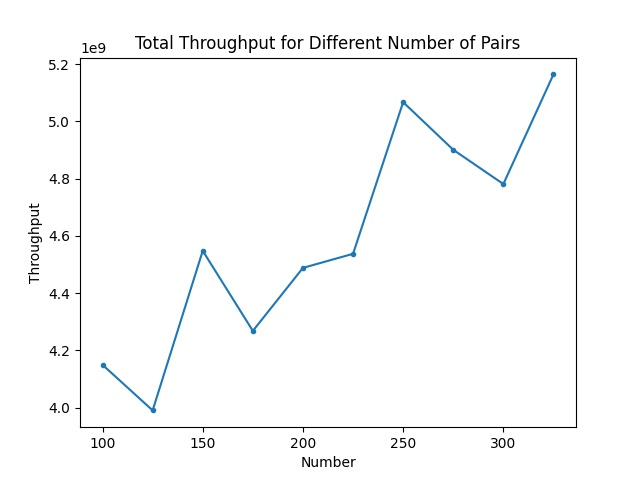
\includegraphics[width=0.45\textwidth]{figbonus_1.jpg}
    \caption{Total Throughput vs. Number of D2D Pair}
    \label{fig:d2d_num_bonus}
\end{figure}
\subsection{Traffic in D2D Simulation}

\subsubsection{Bit Loss Probability in cellular systems}\label{subsub:uldl}
In UL/DL systems, the SINR is huge in contrast to the D2D systems. In the simulation, the data rate is between $100$kbps to $2$Mbps. In \Cref{fig:uplink_sinr}, the median SINR is about 70 dB. By the Shannon Capacity
\begin{equation} \label{eqn:shannon}
    C = BW \times log_2(1 + SINR)
\end{equation}
the rate is approximately $10^6 \times log_2(1+ 10^7) \approx 26$Mbps, which is far faster than the data rate. Therefore, we added a new high data rate of $200$Mbps to test whether the high data rate causes bit loss. Same as expected, the bit loss probability is about $80\%$.
\begin{figure}[htbp]
    \centering
    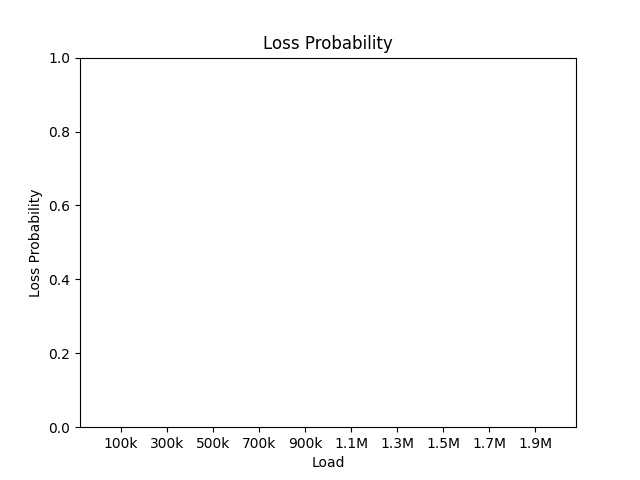
\includegraphics[width=0.45\textwidth]{fig2_1.jpg}
    \caption{Bit Loss Probability of Various Data Rate in cellular systems}
    \label{fig:bit_uldl}
\end{figure}
\subsubsection{Bit Loss Probability in D2D system}\label{subsub:d2d}
\begin{figure}[htbp]
    \centering
    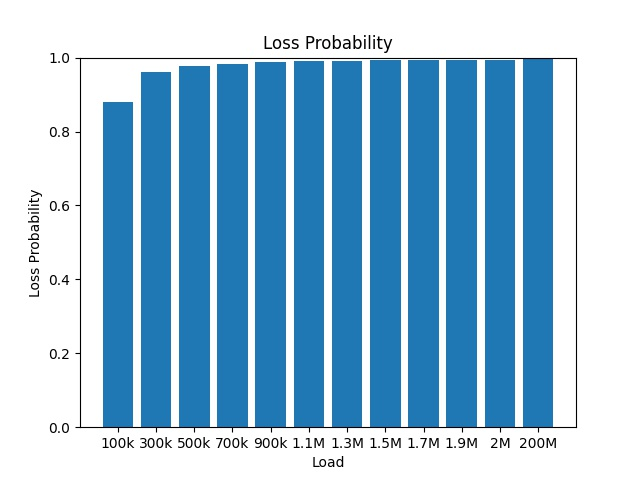
\includegraphics[width=0.45\textwidth]{fig2_2.jpg}
    \caption{Bit Loss Probability of Various Data Rate in D2D systems}
    \label{fig:bit_d2d}
\end{figure}
In \Cref{fig:d2d_sinr}, we have discovered that in D2D systems, the median of SINR is approximately $-25$dB. By \Cref{eqn:shannon}, the transmit rate of the D2D system is about $10^6 \times log_2(1+ 10^{-2.5}) \approx 4.5$kbps, which is far less than the data rate, so the bit loss probability is larger than the cellular scenario. As the data rate increases, the bit loss probability also increases.
\subsection{Traffic in D2D Discussion}
\subsubsection{From the results in \Cref{subsub:uldl} and \Cref{subsub:d2d}, briefly state and explain your observations.}
We stated our observations in \Cref{subsub:uldl} and \Cref{subsub:d2d}.
\subsubsection{Is there any other factors that could affect the performance of cellular and D2D transmission? How?}
The performance of cellular and D2D transmission is mainly based on the interference between other D2D pairs. If there is a power control protocol between each UE, there would be an optimal power control scheme that leads to optimal overall performance.
\subsubsection{Consider the case in which different D2D transmitters have different data arrival rate. If you are required to mitigate the bit loss probability, what would you do?}
First, if the D2D transmitters have different data arrival rate, the slow arrival data rate D2D transmitters would only need small transmit power, and high arrival data rate D2D transmitters can use more power to transmit their data. In other words, if there is a mechanism that can allocate the power usage of all D2D transmitters by their arrival data rate, the interference of other D2D transmitters would decrease. Another way is to allocate different bandwidth to different D2D transmitters by their arrival data rate, so the D2D transmitters with high arrival data rate can use more bandwidth to achieve higher data rate, hence the decline in bit loss probability.
\section{HW6}

\subsection{System Model}
The system is about multicast systems. The number of mobile stations (MS) in each inner base station (BS) is randomly selected from uniform distribution between $[5, 15]$. The base stations will transmit the same data to these mobile stations simultaneously. There are two schemes of multicast. One is Point to Multipoint (PTM), and the other is Single Frequency Network (SFN).

\begin{figure}[htbp]
    \centering
    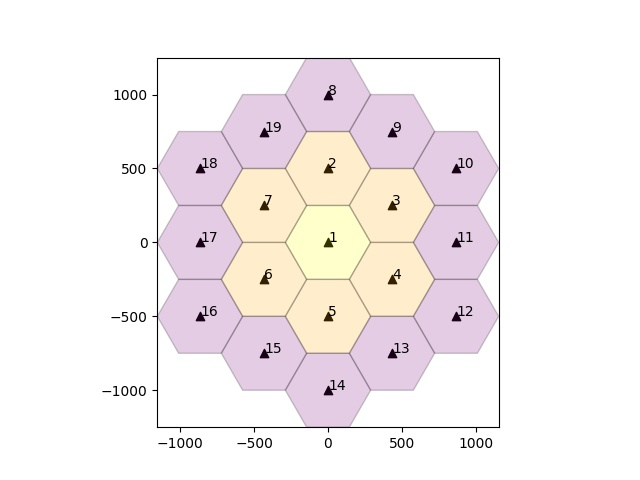
\includegraphics[width=0.45\textwidth]{Cell_ID.jpg}
    \caption{The simulated map for base stations}
    \label{fig:bs_map}
\end{figure}
In \Cref{fig:bs_map}, the orange part is the coverage of seven inner base stations (1-7), while the purple part is the coverage of outer base stations (8-19). We consider the problem that inner BSs multicast to the MSs in inner BSs.
\subsection{Simulation}
\subsubsection{Simulation Parameters}
In the system, the bandwidth is $10$MHz, the temperature is $27^\circ$C, the power of the base stations is $23$dBm, the power of MSs in $0$dBm, the antenna gain of receive and transmit is both $0$dB. The MS height is $1.5$m, and the base station height is $51.5$m. The path loss model is Two-ray-ground model, which has been mentioned in \Cref{eqn:two_ray}.
\subsubsection{Cumulative Distribution of PTM multicast}

\begin{figure}[htbp]
    \centering
    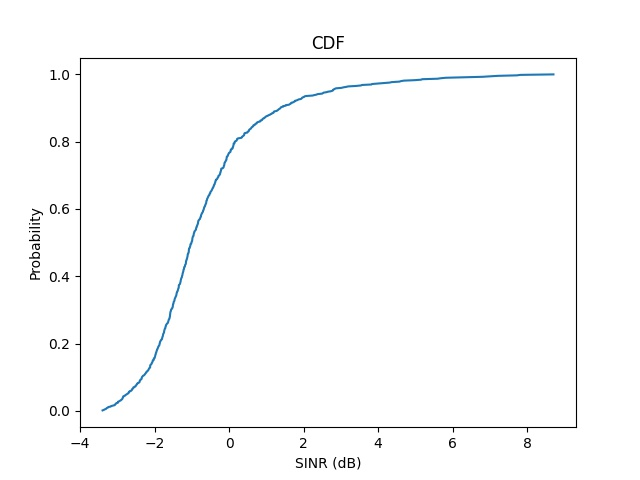
\includegraphics[width=0.45\textwidth]{1-2_CDF.jpg}
    \caption{The CDF of PTM}
    \label{fig:PTM_CDF}
\end{figure}
In the point-to-multipoint multicast network, a single data packet is delivered to multiple mobile stations on a single channel. However, the data rate of the multicast transmission is limited by the mobile station with the poorest channel quality in the base station.

The cumulative distribution of the PTM multicast ranges around -4 to 4 decibels. As shown in \Cref{fig:PTM_CDF}, most of the poorest signal-to-interference-plus-noise ratios (SINR) appear to range between -2 to 0 dB, approximately peaking at -1.5 dB.

\subsubsection{Average Data Rate and Resource Efficiency for PTM}
We calculated the average data rate and the resource efficiency for PTM. For every inner base station, we obtained the transmission data rate from the poorest SINR by calculating it from \cref{eqn:shannon} and multiplied by the MSs number within the cell. After looping over 100 times, the data rates are summed up and divided by the total number of MSs in the simulation. The resource efficiency is computed from the average of the received data rate in each iteration divided by the bandwidth.
\\
\\
Average data rate of PTM: $768483.2746327275$ bits/s\\
Average resource efficiency of PTM: $63.660515107604226$

\subsubsection{Cumulative Distribution of SFN multicast}

\begin{figure}[htbp]
    \centering
    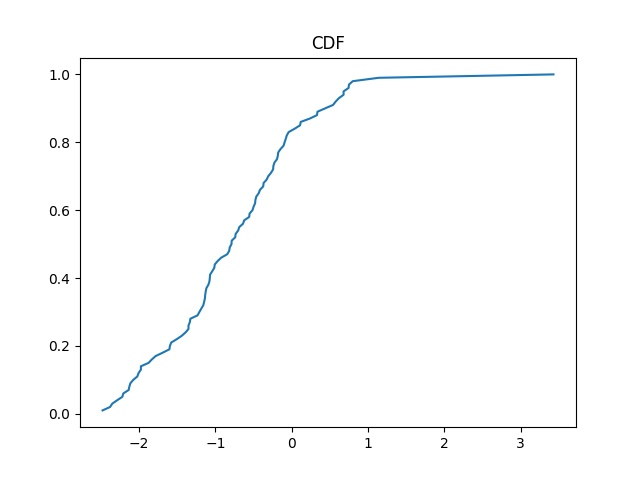
\includegraphics[width=0.45\textwidth]{2-1_CDF.jpg}
    \caption{The CDF of SFN}
    \label{fig:SFN_CDF}
\end{figure}
In SFN multicast, the inner BSs cooperate with each other. They transmit the
same data packet on the same $10$MHz band simultaneously. Hence, the signals reaching MSs become constructive and the signals from outer BSs remain interference. Different from the PTM case, the bottleneck data transmission rate is the one with the poorest channel quality in the coverage of the $7$ inner BSs.

We run the simulation time for $100$ times. In each iteration, we can obtain the poorest SINR among all MSs and plot a figure of CDF. As shown in \Cref{fig:SFN_CDF}, the poorest SINR of the mobile stations ranges from -3 to 3 dB.
\subsubsection{Average Data Rate and Resource Efficiency for SFN}
In the last section, we can also obtain the number of MSs. We use the poorest SINR to calculate the bottleneck data rate by \Cref{eqn:shannon}. Since the inner BSs multicast with the bottleneck data rate to all the MSs, we multiply the bottleneck data rate with the number of MSs and then divided by bandwidth to acquire the resource efficiency. The average data rate and resource efficiency of 100 iterations are as follows.
\\
\\
Average data rate of SFN: $593148.1558335794$ bits/s\\
Average resource efficiency of SFN: $62.3895170645104$
\subsection{PTM and SFN Multicast Performance Discussion}
Based on the default setting, the resource efficiency of PTM and SFN are similar. We have tried several number of MSs and found that the resource efficiency of SFN becomes better than the one of PTF when the number of MSs increases. Hence, SFN performs better when the number of MSs is large. We will provide the resource efficiency and data rate under different conditions. The result is shown as \Cref{table:Data Rate&Resource Efficiency under different conditions}.
\begin{table}[]
\begin{tabular}{|c|c|c|c|c|}
\hline
\begin{tabular}[c]{@{}c@{}}Number of MSs\\ in each cell\end{tabular} &
  \begin{tabular}[c]{@{}c@{}}Resource \\ Efficiency\\ (PTM)\end{tabular} &
  \begin{tabular}[c]{@{}c@{}}Resource \\ Efficiency\\ (SFN)\end{tabular} &
  \begin{tabular}[c]{@{}c@{}}Data Rate\\ (PTM)\end{tabular} &
  \begin{tabular}[c]{@{}c@{}}Data Rate\\ (SFN)\end{tabular} \\ \hline
1$\sim$5     & 32.65  & 25.32  & 9507997bit/s & 5950838bit/s \\ \hline
10$\sim$15   & 73.01  & 73.75  & 600959bit/s  & 603936bit/s  \\ \hline
20$\sim$25   & 119.34 & 125.57 & 330055bit/s  & 347124bit/s  \\ \hline
30$\sim$35   & 162.92 & 172.49 & 238384bit/s  & 252546bit/s  \\ \hline
100$\sim$105 & 453.47 & 501.23 & 60772bit/s   & 67169bit/s   \\ \hline
\end{tabular}
\caption{Data Rate and Resource Efficiency under different conditions}
\label{table:Data Rate&Resource Efficiency under different conditions}
\end{table}

From \cref{table:Data Rate&Resource Efficiency under different conditions}, it is obvious that the resource efficiency and data rate of SFN exceed the ones of PTM when the number of MSs in each cell is larger than 10-15. Therefore, the conclusion is that PTM performs better than SFN when number of MSs is small and worse when number of MSs is large.
We speculate a possible reason. When the number of MSs in each cell increase, the probability of the distance from the farthest MS to BS becomes large in the cell also increases.
In PTM mode, the received SINR in BS i is as follow.
\begin{equation}\label{eqn:SINR in PTM}
    SINR_i = \frac{S_i}{\sum_{k\neq{i}}S_k+N}
\end{equation}
, where $S_k$ is the received signal from BS k and $N$ is noise.
In SFN mode, the received SINR in BS i is as follow.
\begin{equation}\label{eqn:SINR in SFN}
    SINR_i = \frac{\sum_{k=1}^{7}S_k}{\sum_{k=8}^{19}S_k+N}
\end{equation}
, where $S_k$ is the received signal from BS k and $N$ is noise.

When the distance between MS and BS is small, the signal from its BS is much stronger than any other BSs, so the difference of SINR between PTM mode and SFN mode is small. That is, they have almost identical SINR if the distance between MS and BS is small.

Under the condition of fewer MSs in each cell, the farthest MS is nearer to the BS comparing to more MSs. As mentioned above, the SINR in both two modes is similar if the MS is near the BS. In PTM mode, the bottleneck SINR is to pick the MS with the poorest SINR in each inner cell respectively. In SFN, the bottleneck SINR is to pick the MS with the poorest SINR in all of the inner cells. The latter must be poorer than the former, which results in better performance in PTM when the number of MSs is small.

When the distance between MS and BS is large, the signal from its BS is not so dominant as the case of short distance, so the signals from other BSs play a more significant mode when calculating SINR. The SINR of SFN will larger than the one of PTM. The larger distance between MS and BS is, the larger difference between the SINR of both two modes is. In other words, The poorest SINR of SFN is larger than the one of PTM if the distance between MS and BS is large.

To sum up, the number of MSs determines the distance between the farthest MS to its BS, which directly infect the poorest SINR of PTM and SFN modes respectively. The larger of poorest SINR is, the higher the performance is. The conclusion can explain the phenomenon of the data we collect above.

\section{Conclusion}
In the first section, we simulated and discussed the difference between D2D systems and cellular systems. In the second section, the PTM and the SFN multicast are simulated. We concluded that the number of MSs influences resource efficiency due to the SINR probability.
\end{document}
